\chapter{Практическая часть}

В данной главе рассматривается  практическое приложение метода квантовых состояний нейронной сети к 
нахождению основного состояния ансамбля спинов, характеризуемых некоторыми классическими гамильтонианами.
Приводятся результаты обучения искусственной нейронной сети и их анализ.

\section{Исследуемые гамильтонианы}

В данной работе будут рассмотрены два классических гамильтониана с известными значениями энергии основного состояния цепочки $N=20$ спинов и изотропная часть гамильтониана магнитного кластера $\text{V}_{15}$.

Первым классическим гамильтонианом является модель Изинга поперечного поля:

\begin{equation}
\hat{\mathcal{H}}_\text{TFI}=-h\sum_{i}\hat{\sigma}_i^x-J_z\sum_{\langle i,j\rangle}\hat{\sigma}_i^z \hat{\sigma}_j^z
\end{equation}

\noindent где в данной работе $h=J_z=1$.

Вторым классическим гамильтонианом является модель антиферромагнетика Гейзенберга:

\begin{equation}
\hat{\mathcal{H}}_\text{AFH}=\sum_{\langle i,j\rangle}\hat{\sigma}_i^x \hat{\sigma}_j^x+\hat{\sigma}_i^y \hat{\sigma}_j^y+J_z\hat{\sigma}_i^z \hat{\sigma}_j^z
\end{equation}

\noindent где в данной работе $J_z=1$.

Изотропная часть гамильтониана магнитного кластера $\text{V}_{15}$ \cite{konstantinidis2002magnetic}:
\begin{equation}
\hat{\mathcal{H}}_\text{V$_{15}$}=\hat{\mathcal{H}}_0+\hat{\mathcal{H}}_1
\end{equation}

\begin{equation*}
\hat{\mathcal{H}}_0=\frac{1}{4}J(\hat{\boldsymbol{\sigma}}_1 \cdot \hat{\boldsymbol{\sigma}}_2 + \hat{\boldsymbol{\sigma}}_3 \cdot \hat{\boldsymbol{\sigma}}_4 + \hat{\boldsymbol{\sigma}}_5 \cdot \hat{\boldsymbol{\sigma}}_6 + \hat{\boldsymbol{\sigma}}_{10} \cdot \hat{\boldsymbol{\sigma}}_{11} + \hat{\boldsymbol{\sigma}}_{12} \cdot \hat{\boldsymbol{\sigma}}_{13} + \hat{\boldsymbol{\sigma}}_{14} \cdot \hat{\boldsymbol{\sigma}}_{15})
\end{equation*}

\begin{equation*}
\begin{split}
\hat{\mathcal{H}}_1=\frac{1}{4}&J'(\hat{\boldsymbol{\sigma}}_2 \cdot \hat{\boldsymbol{\sigma}}_3 + \hat{\boldsymbol{\sigma}}_4 \cdot \hat{\boldsymbol{\sigma}}_5 + \hat{\boldsymbol{\sigma}}_1 \cdot \hat{\boldsymbol{\sigma}}_6 + \hat{\boldsymbol{\sigma}}_{11} \cdot \hat{\boldsymbol{\sigma}}_{12} + \hat{\boldsymbol{\sigma}}_{13} \cdot \hat{\boldsymbol{\sigma}}_{14} + \hat{\boldsymbol{\sigma}}_{10} \cdot \hat{\boldsymbol{\sigma}}_{15})+\\
+\frac{1}{4}&J''(\hat{\boldsymbol{\sigma}}_1 \cdot \hat{\boldsymbol{\sigma}}_3 + \hat{\boldsymbol{\sigma}}_3 \cdot \hat{\boldsymbol{\sigma}}_5 + \hat{\boldsymbol{\sigma}}_1 \cdot \hat{\boldsymbol{\sigma}}_5 + \hat{\boldsymbol{\sigma}}_{10} \cdot \hat{\boldsymbol{\sigma}}_{12} + \hat{\boldsymbol{\sigma}}_{12} \cdot \hat{\boldsymbol{\sigma}}_{14} + \hat{\boldsymbol{\sigma}}_{10} \cdot \hat{\boldsymbol{\sigma}}_{14}) + \\
+\frac{1}{4}&J_1 (\hat{\boldsymbol{\sigma}}_2 \cdot \hat{\boldsymbol{\sigma}}_7 + \hat{\boldsymbol{\sigma}}_7 \cdot \hat{\boldsymbol{\sigma}}_{11} + \hat{\boldsymbol{\sigma}}_4 \cdot \hat{\boldsymbol{\sigma}}_8 + \hat{\boldsymbol{\sigma}}_{8} \cdot \hat{\boldsymbol{\sigma}}_{15} + \hat{\boldsymbol{\sigma}}_{6} \cdot \hat{\boldsymbol{\sigma}}_{9} + \hat{\boldsymbol{\sigma}}_{9} \cdot \hat{\boldsymbol{\sigma}}_{13}) + \\
+\frac{1}{4}&J_2 (\hat{\boldsymbol{\sigma}}_1 \cdot \hat{\boldsymbol{\sigma}}_7 + \hat{\boldsymbol{\sigma}}_7 \cdot \hat{\boldsymbol{\sigma}}_{10} + \hat{\boldsymbol{\sigma}}_3 \cdot \hat{\boldsymbol{\sigma}}_8 + \hat{\boldsymbol{\sigma}}_{8} \cdot \hat{\boldsymbol{\sigma}}_{14} + \hat{\boldsymbol{\sigma}}_{5} \cdot \hat{\boldsymbol{\sigma}}_{9} + \hat{\boldsymbol{\sigma}}_{9} \cdot \hat{\boldsymbol{\sigma}}_{12})
\end{split}
\end{equation*}

\noindent где в данной работе используются следующие параметры:

\[
J=800\ \text{K},\ J'=J_1=350\ \text{K},\ J''=J_2=225\ \text{K}
\]

\section{Результаты обучения нейронной сети}

Результаты обучения ограниченной машины Больцмана на модели Изинга поперечного поля представлены на рис. \ref{fig:energyisingmodel}. Здесь для SGD в качестве параметров использовались:

\[
\alpha=10^{-2},\ \epsilon_0=100,\ b=0,9,\ \epsilon_{\min}=10^{-4}
\]

\begin{figure}[b!]
    \centering
    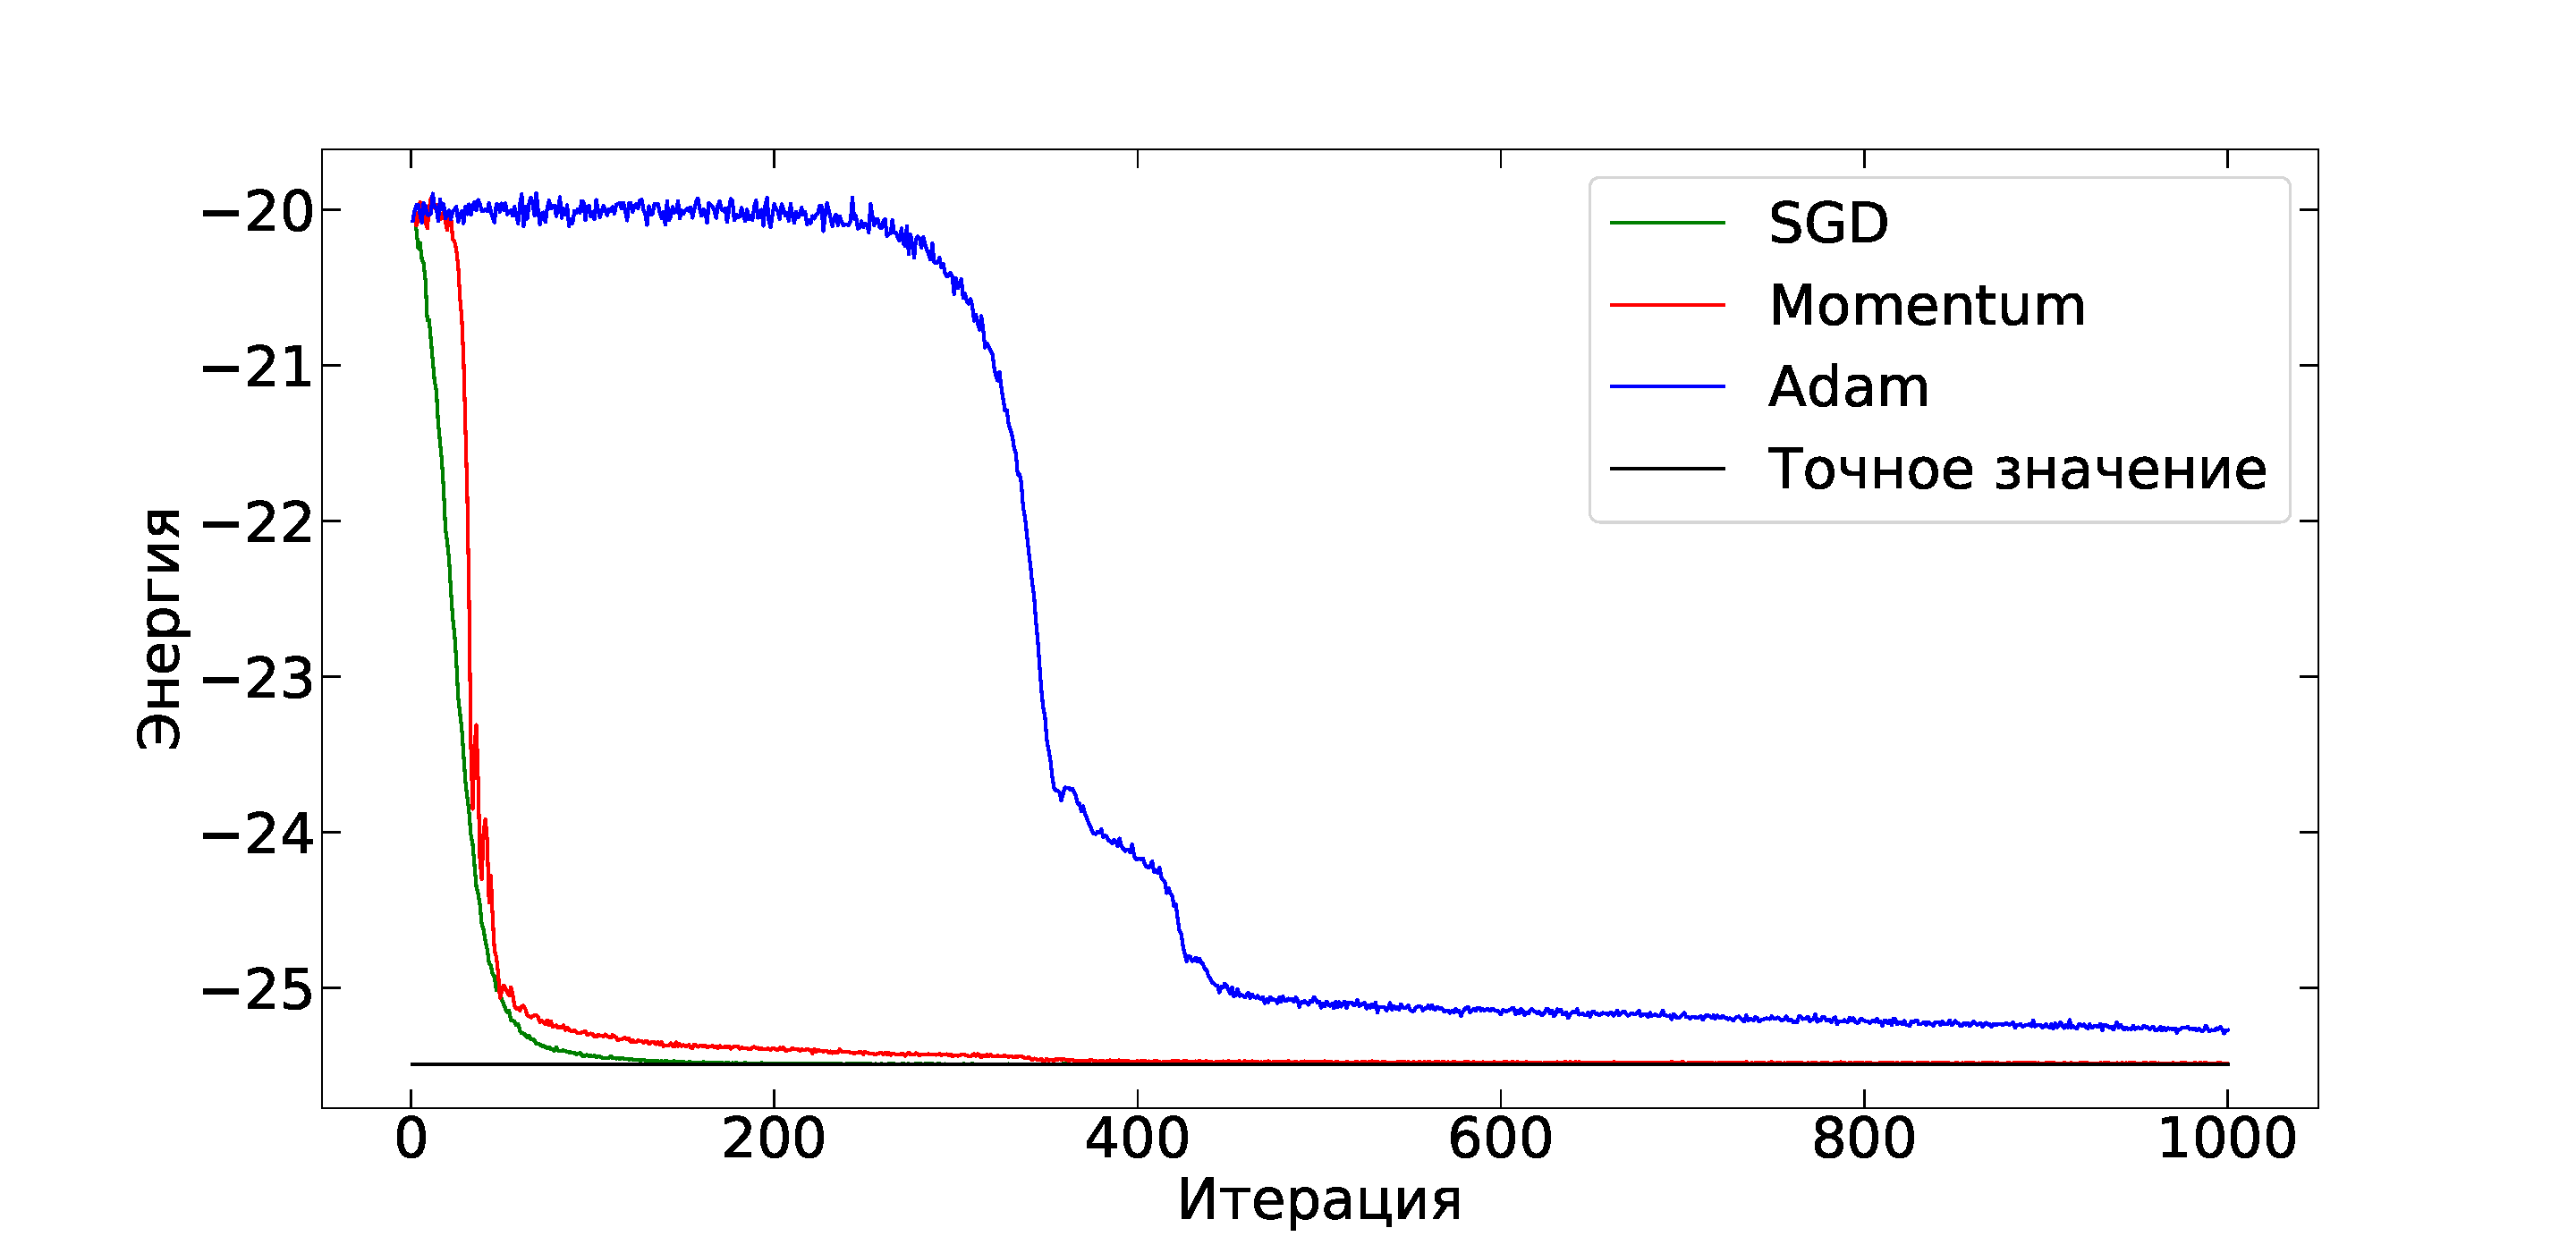
\includegraphics[width=\linewidth]{pictures/energy_ising_model}
    \caption[]{Результат обучения на модели Изинга поперечного поля}
    \label{fig:energyisingmodel}
\end{figure}

Как видно из рис. \ref{fig:errorisingmodel} SGD отлично подошел в качестве метода решения для данного гамильтониана, достигнув относительной погрешности менее 0,01\%. 
Модификации данного метода с такими же значениями скорости обучения не смогли похвастаться такой же точностью. 
И если Momentum еще показывает убедительную сходимость, то Adam смог достигнуть только 1\% относительной погрешности. 
Здесь стоит оговориться, что, как выяснилось в дальнейшем, это результат удачного подбора регуляризационных параметров при вычислении стохастической матрицы реконфигурации.
При этом Adam показывает свой характер сходимости, а именно длительное накапливание   градиента, и затем стремительное повышение точности.
При этом Adam более устойчив в плане параметров обучения.
Таким образом, довольно медленное и устойчивое продвижение к минимуму и меньшая зависимость от выбранных параметров выгодно отличает его от других более чувствительных методов. 

Результаты обучения ограниченной машины Больцмана на модели антиферромагнетика Гейзенберга представлены на рис. \ref{fig:energyheisenbergmodel}. Здесь для SGD в качестве параметров использовались те же регуляризационные параметры, а значение скорости обучения составило:

\[
\alpha=10^{-3}
\]

\begin{figure}[t!]
    \centering
    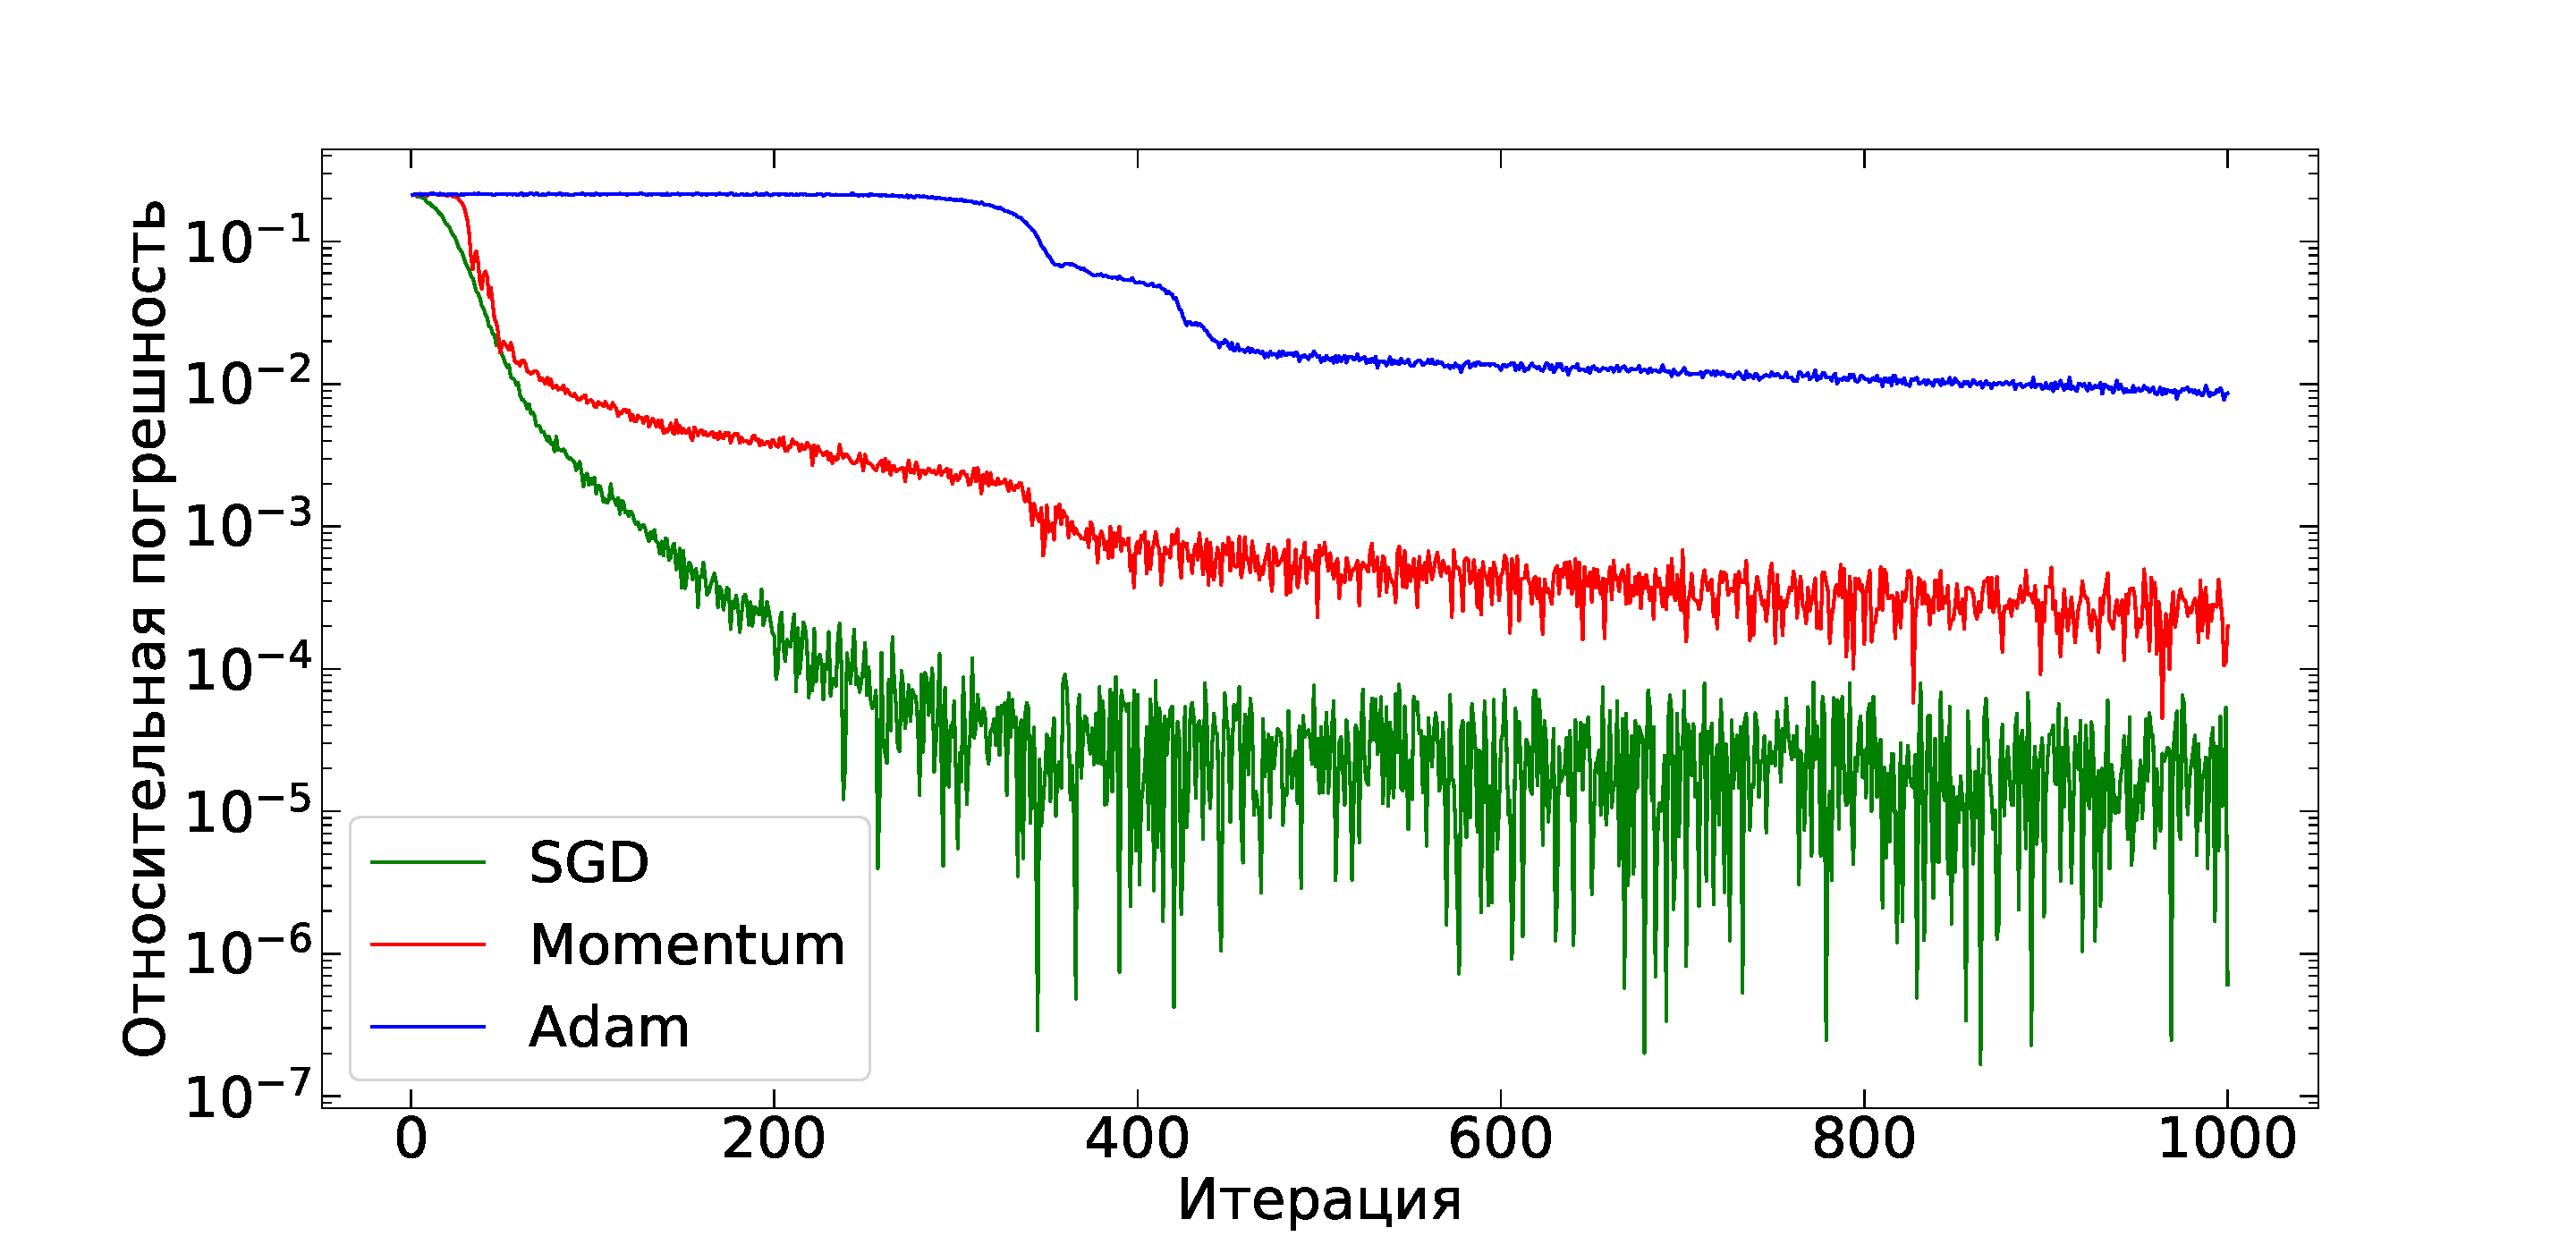
\includegraphics[width=\linewidth]{pictures/error_ising_model}
    \caption[]{Точность обучения на модели Изинга поперечного поля}
    \label{fig:errorisingmodel}
\end{figure}

\begin{figure}[]
    \centering
    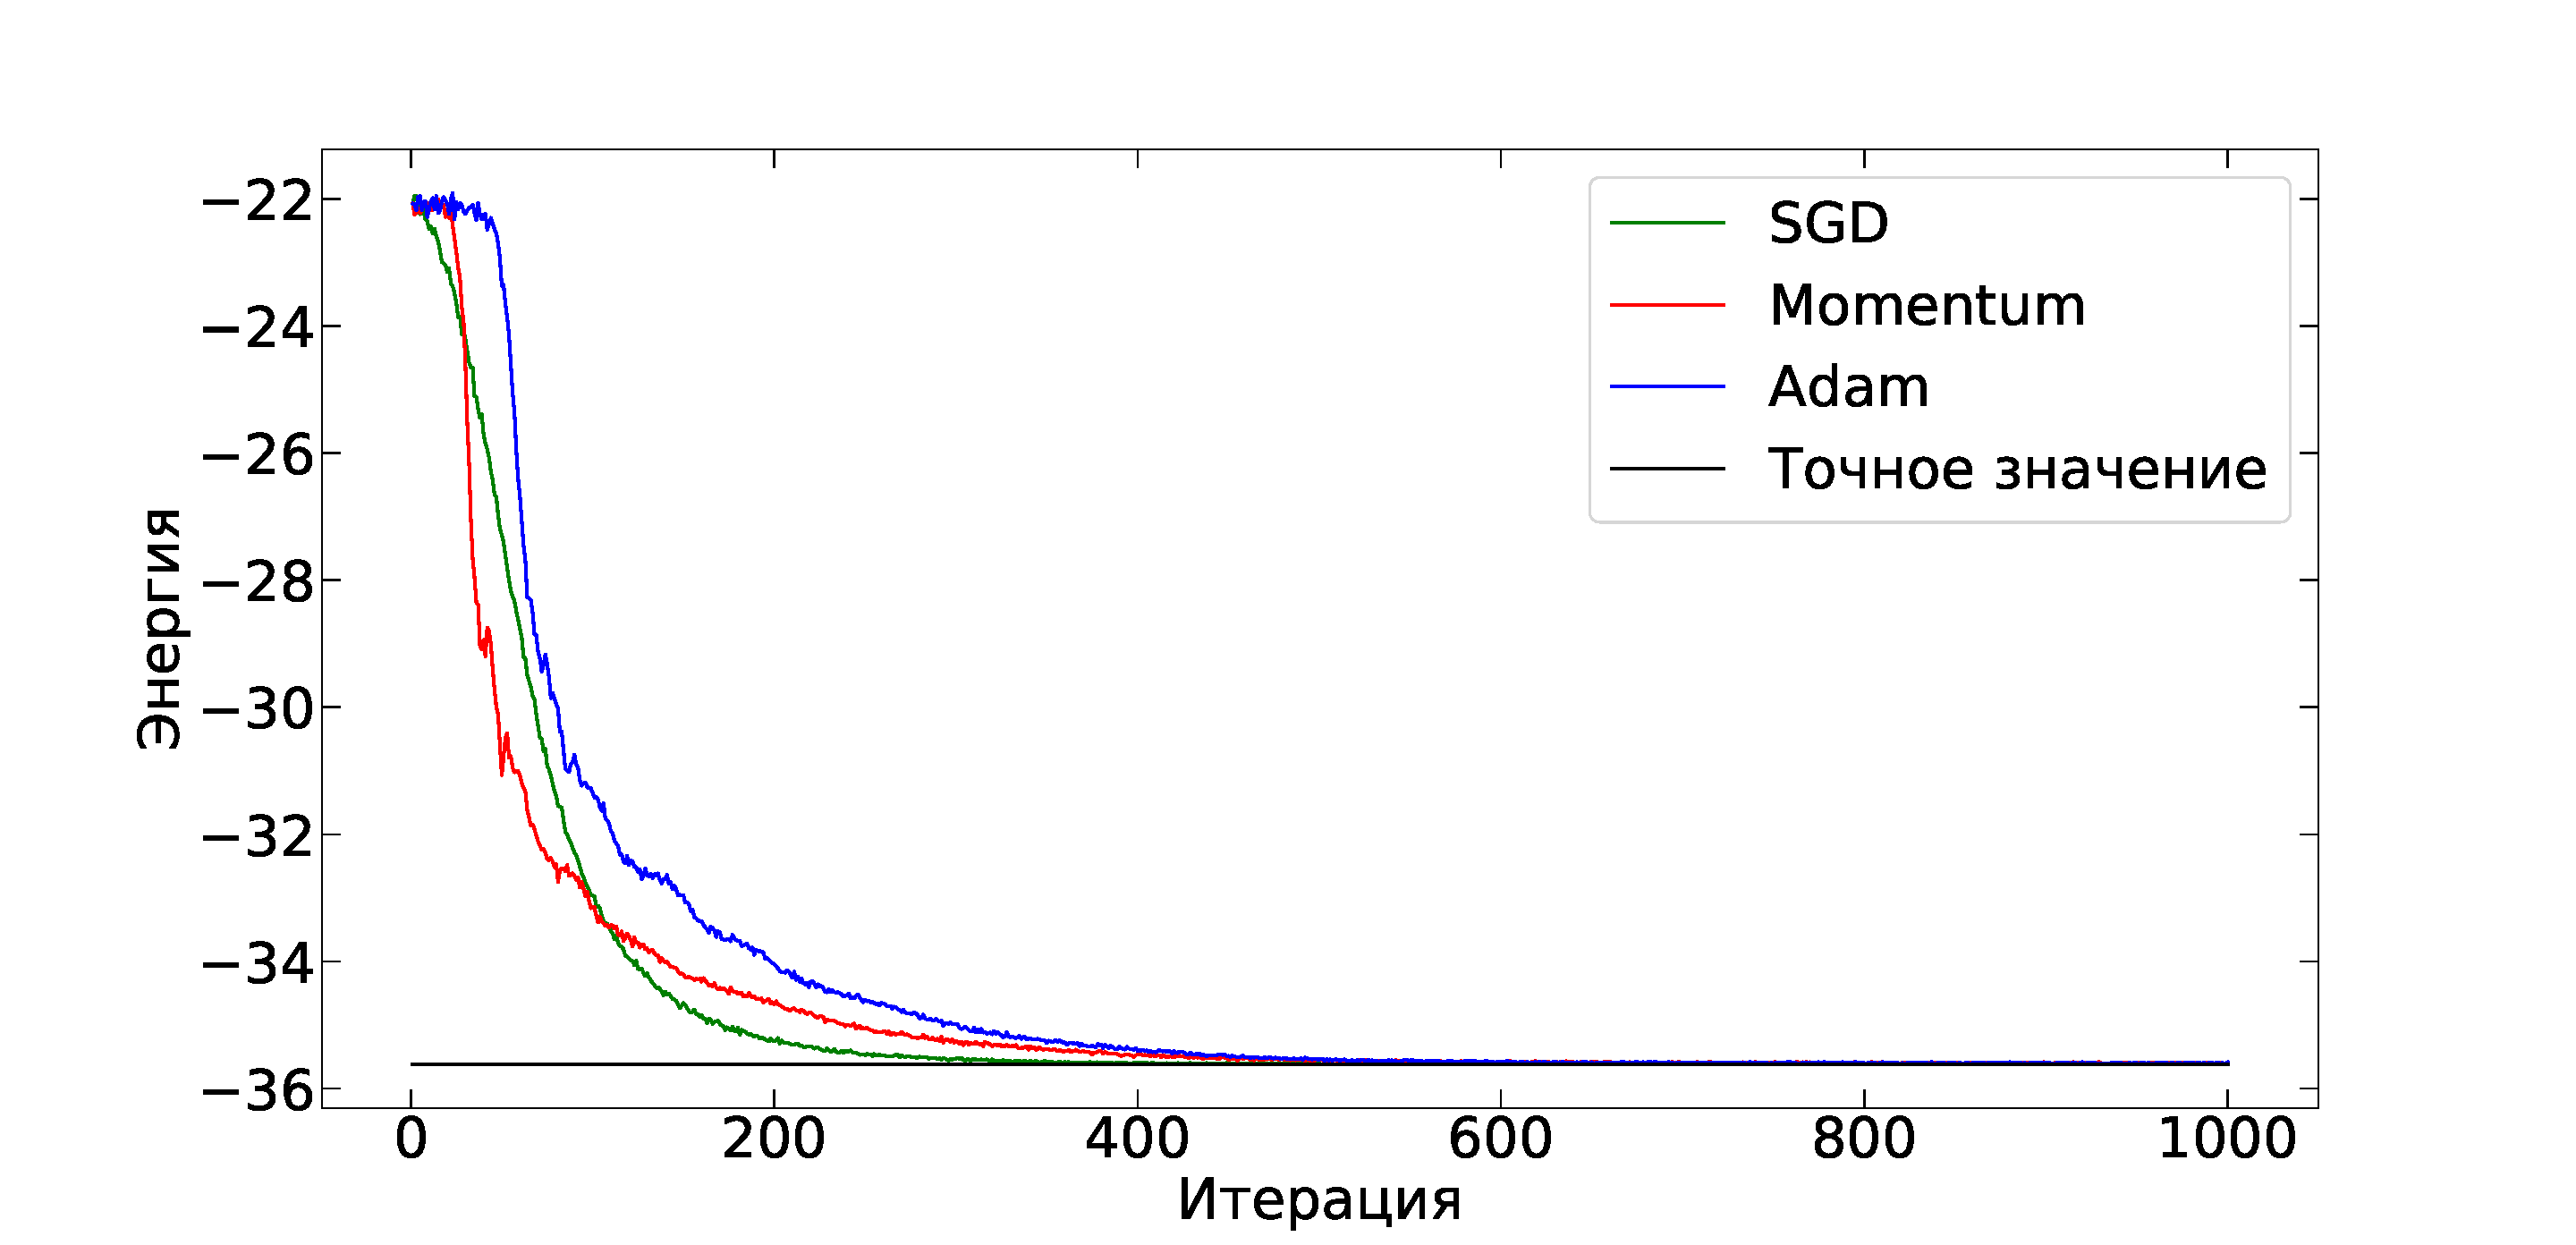
\includegraphics[width=\linewidth]{pictures/energy_heisenberg_model}
    \caption[]{Результат обучения на модели антиферромагнетика Гейзенберга}
    \label{fig:energyheisenbergmodel}
\end{figure}

Как видно из рис. \ref{fig:errorheisenbergmodel} SGD по-прежнему достиг относительной погрешности менее 0,01\%. 
Модификации данного метода обладали следующими скоростями обучения:

\begin{equation*}    
\begin{split}
\text{Momentum}:&\ \alpha=5\cdot 10^{-3}\\
\text{Adam}:&\ \alpha=0,1\\
\end{split}
\end{equation*}

\begin{figure}[b!]
    \centering
    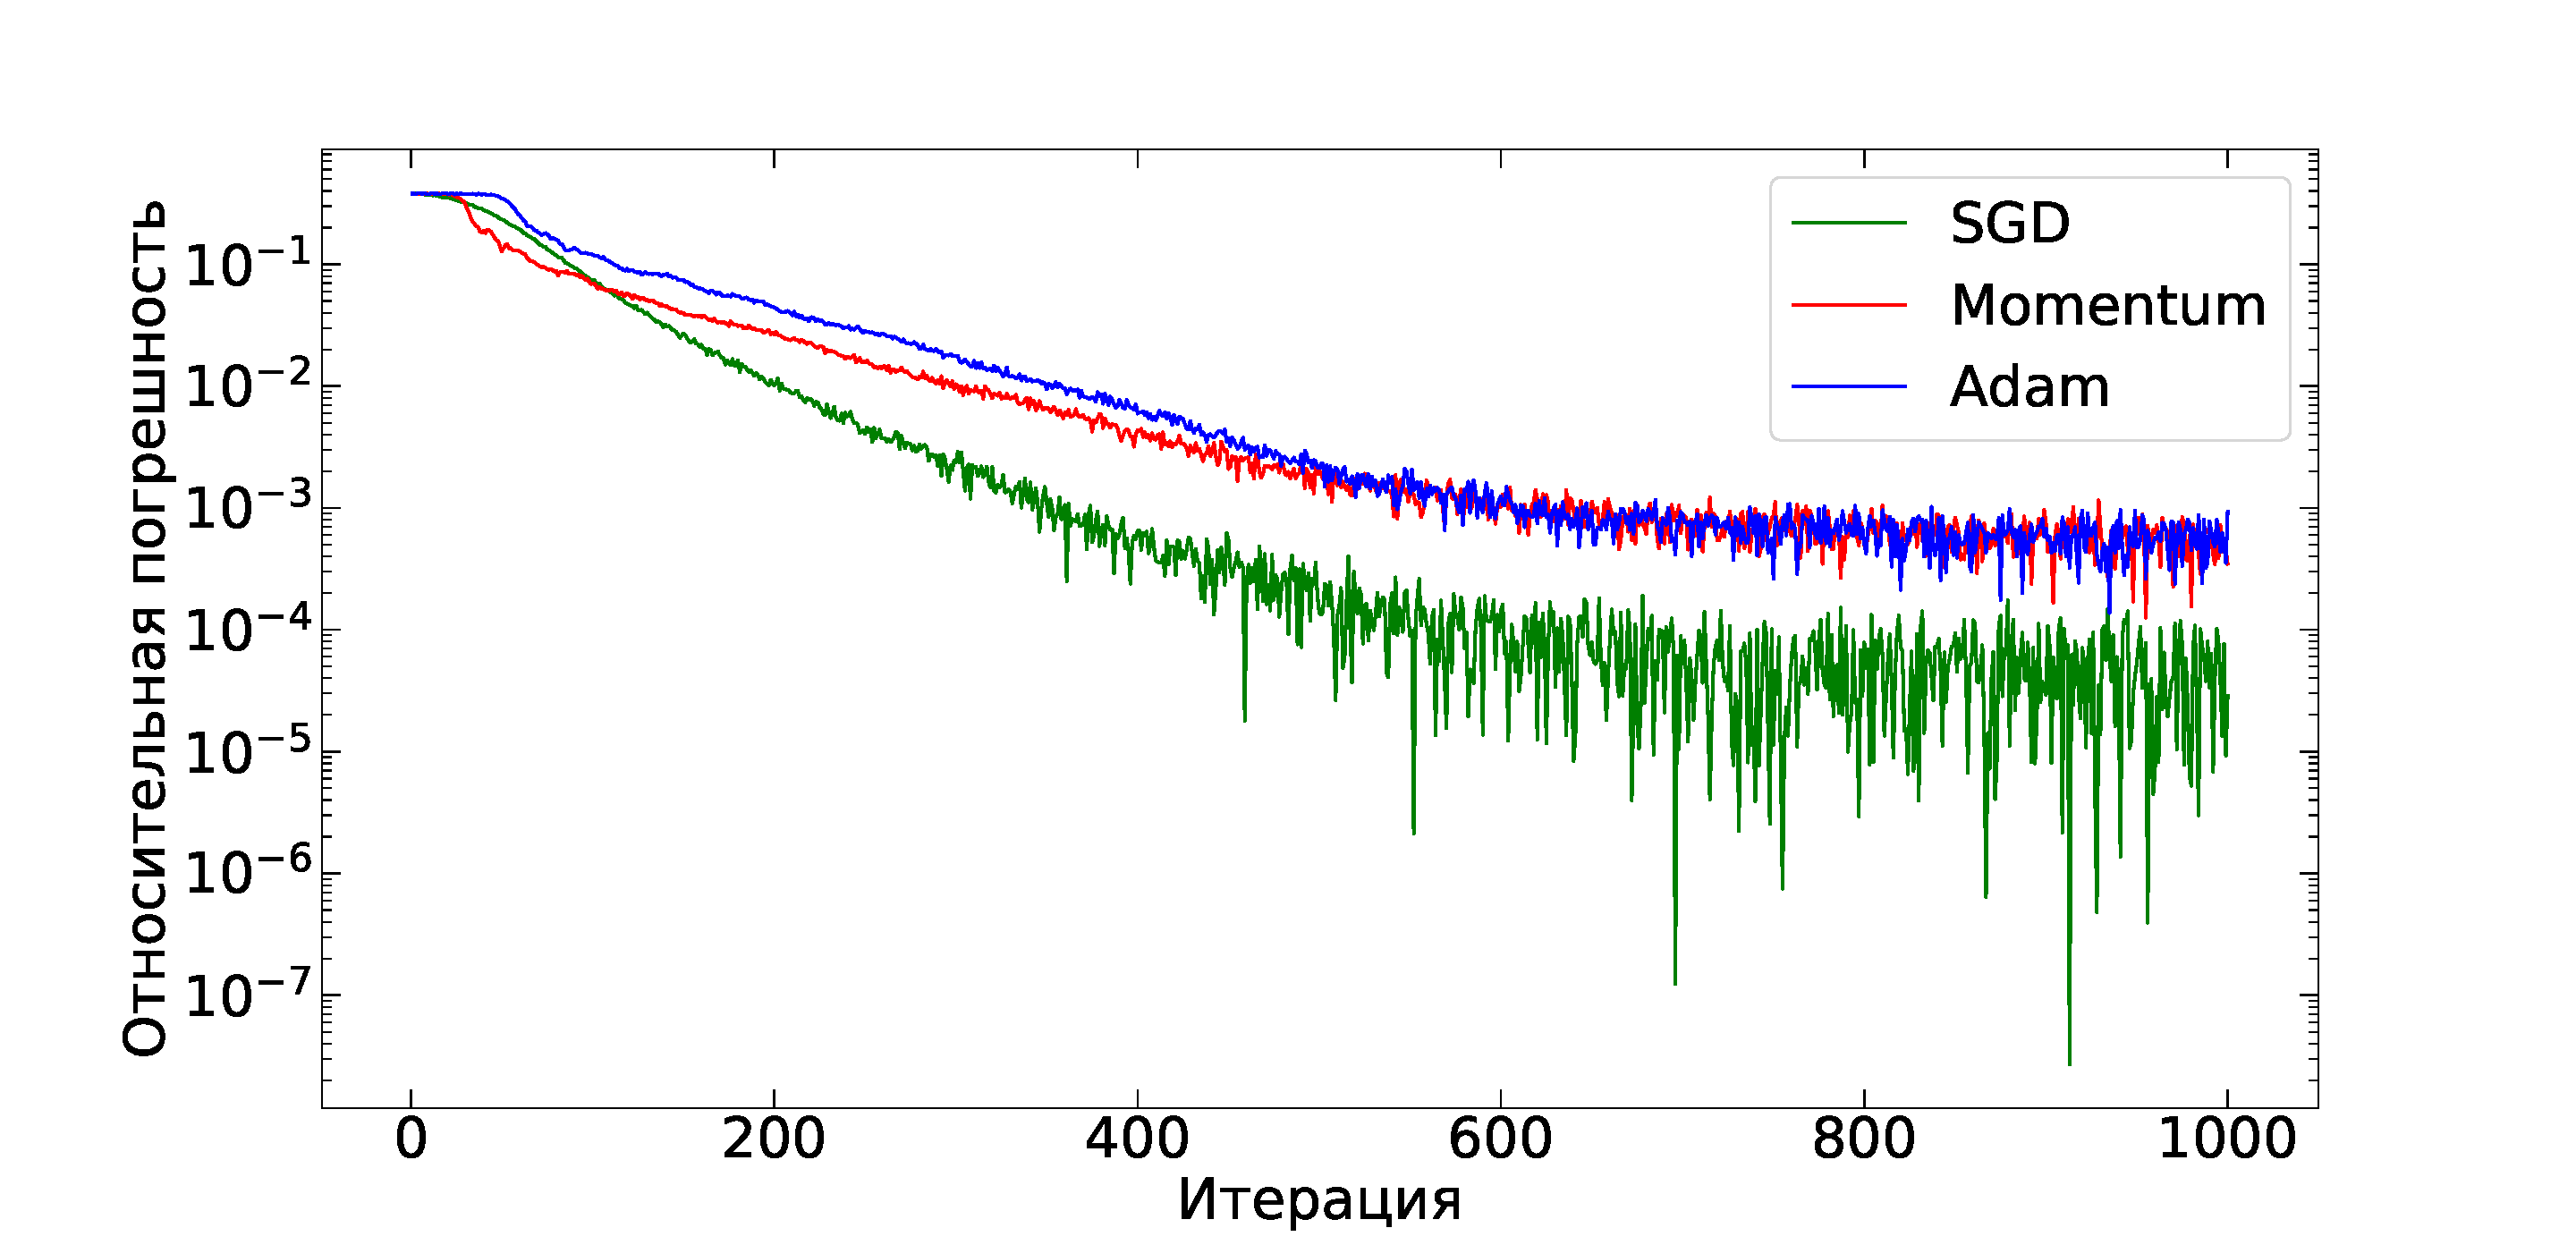
\includegraphics[width=\linewidth]{pictures/error_heisenberg_model}
    \caption[]{Точность обучения на модели антиферромагнетика Гейзенберга}
    \label{fig:errorheisenbergmodel}
\end{figure}

Здесь становится заметно преимущество модификаций перед стандартным SGD.
Так, Momentum и Adam уже не так сильно отстают.
При этом учитывая, что скорость обучения фиксирована, становиться понятно, почему SGD не уступает лидерство.
При уменьшении скорости обучения SGD бы попал в локальный минимум, в то время как Adam и Momentum, обладая большим запасом градиента, еще некоторое время двигались бы в поисках глобального минимума. 
Но в данной работе это не рассматривается, так как такой глубокий поиск невозможен без автоматического поиска подходящих параметров обучения.
Пока же критерии поиска не выработаны, автоматизировать данную операцию не представляется выгодным по времени.
Так что пока основным методом является исследование с постоянной скоростью обучения возможных кандидатов на глобальный минимум, обладающих достаточной устойчивостью при обучении, при рекомендуемых значениях параметров.

\begin{figure}
    \centering
    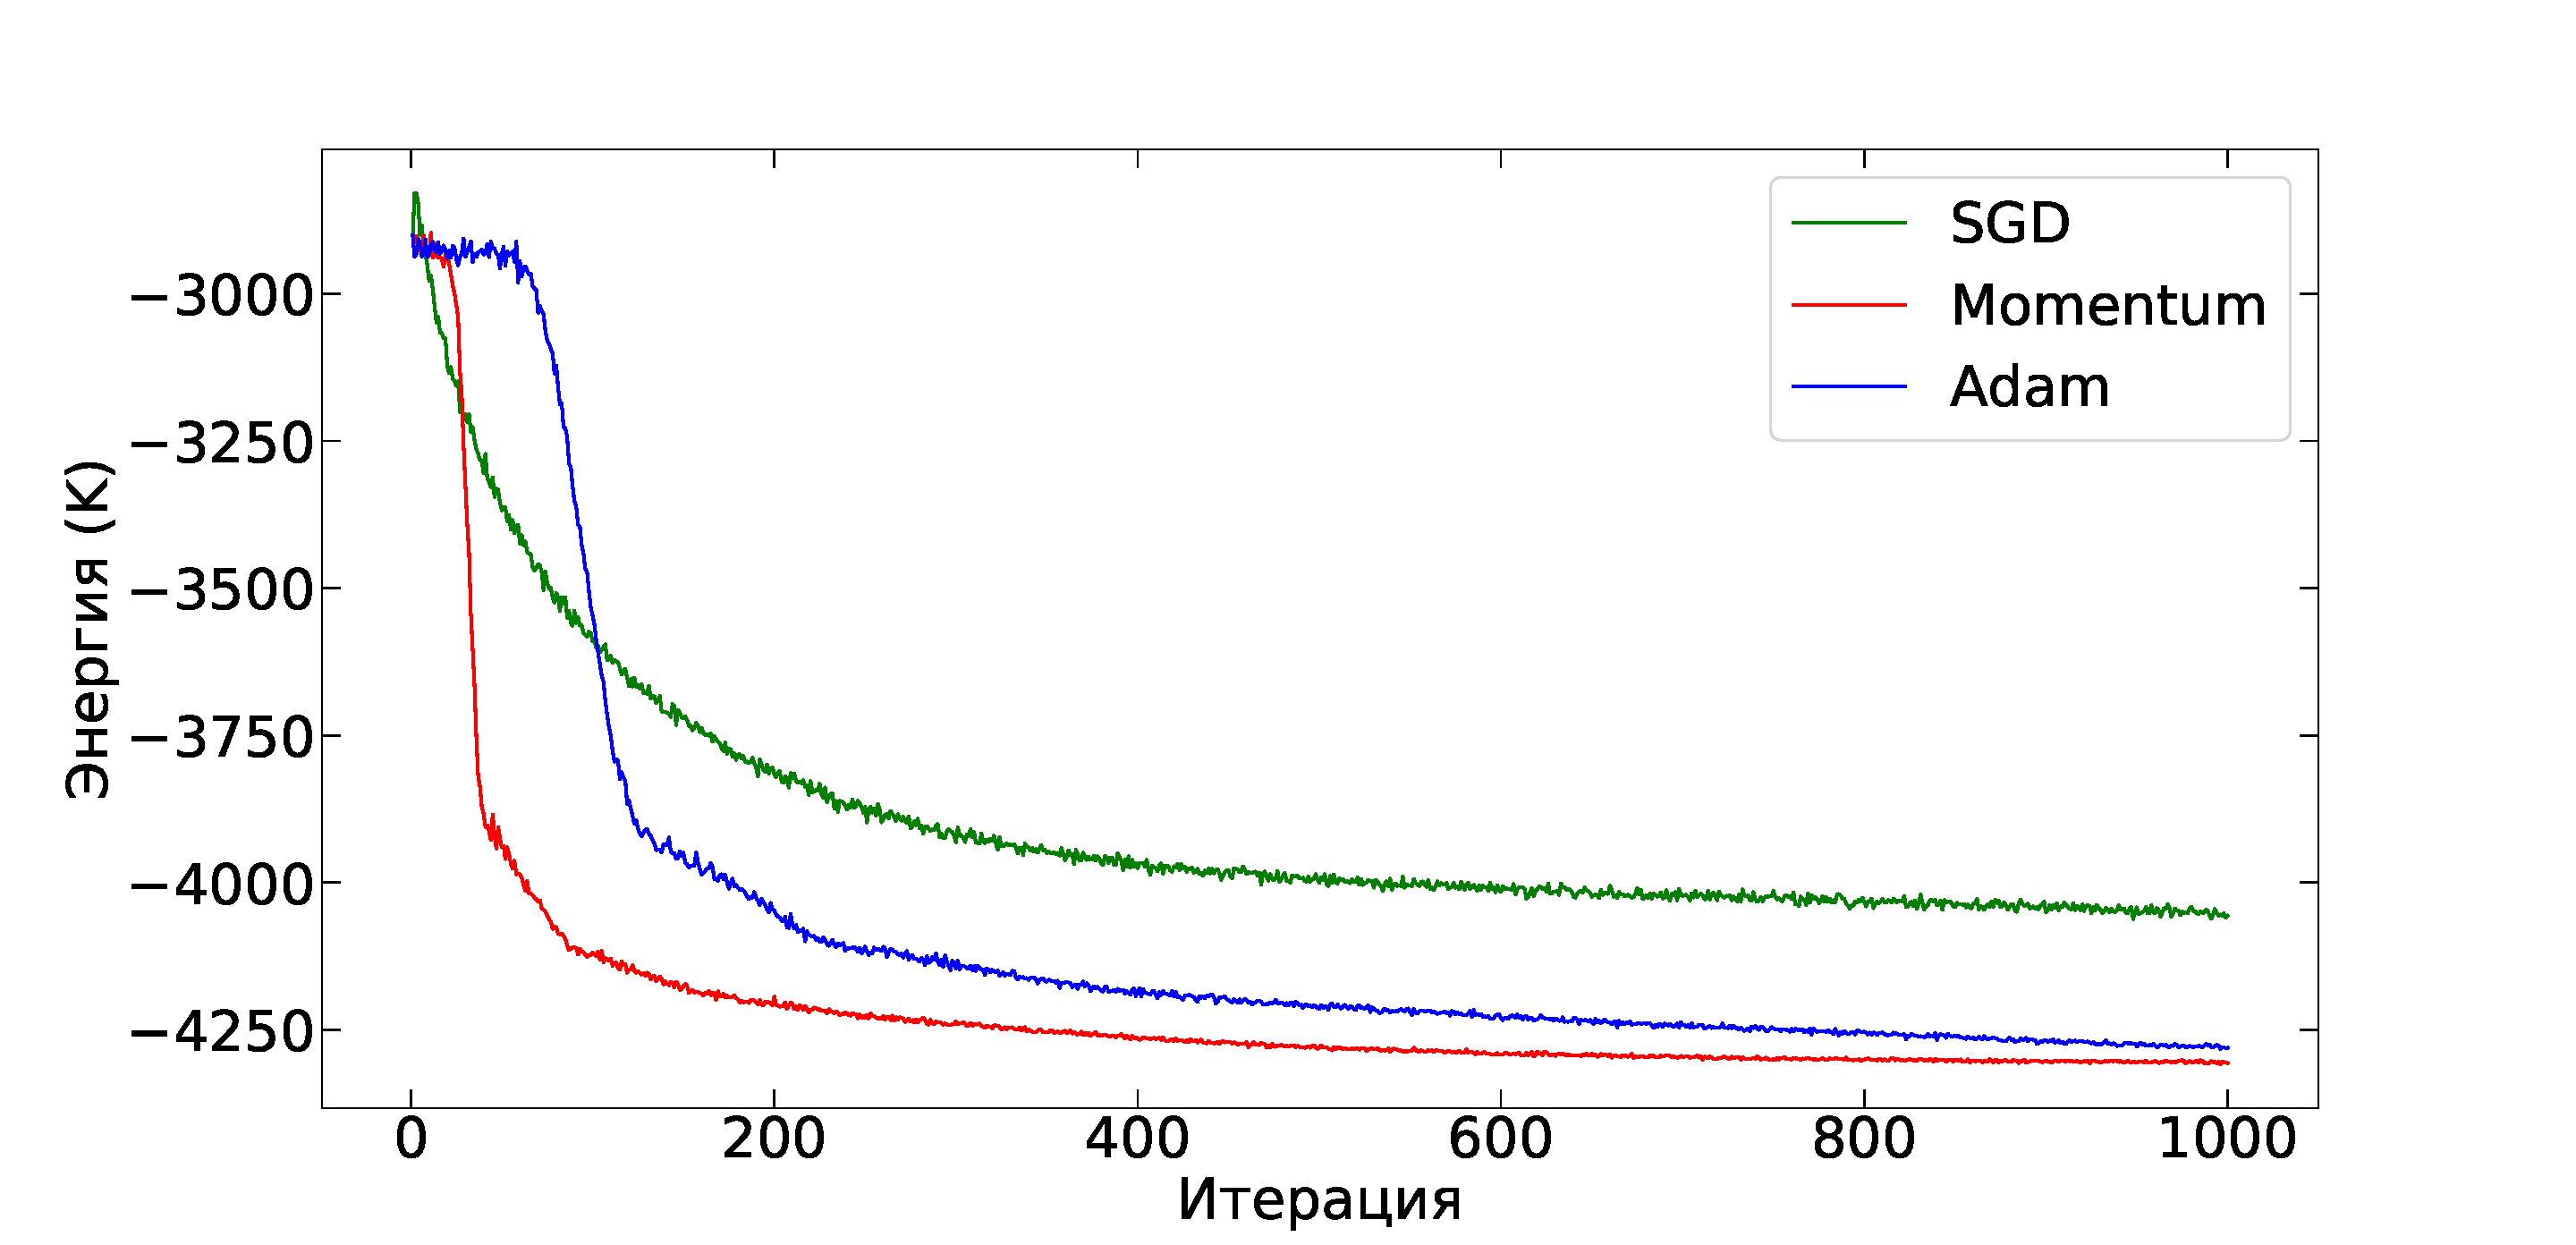
\includegraphics[width=\linewidth]{pictures/energy_v15_isotropic}
    \caption[]{Результат обучения на изотропной части гамильтониана магнитного кластера $\text{V}_{15}$}
    \label{fig:energyv15isotropic}
\end{figure}

Результаты обучения ограниченной машины Больцмана на изотропной части гамильтониана магнитного кластера  $\text{V}_{15}$ представлены на рис. \ref{fig:energyv15isotropic}. Здесь для методов оптимизации в качестве параметров обучения использовались:

\begin{equation*}    
\begin{split}
\text{SGD}:&\ \alpha=5\cdot 10^{-5},\ \epsilon_0=100,\ b=0,999,\ \epsilon_{\min}=20\\
\text{Momentum}:&\ \alpha=5\cdot 10^{-5}\\
\text{Adam}:&\ \alpha=5\cdot 10^{-4}\\
\end{split}
\end{equation*}

Именно для системы спинов с нетривиальными взаимодействиями проявилась проблема подбора параметров для простейших методов оптимизации.
Старые параметры не подходят, так как с ними происходит срыв обучения.
Поэтому правильность их подбора и определяет сходимость простейших методов.
Данные параметры для SGD, как видно из результатов обучения, не являются оптимальными, так как обучение ограниченной машины Больцмана происходит медленно.
Оптимальные параметры для нетривиальных взаимодействий уже намного труднее правильно подобрать, 
в то время как рекомендуемые для большинства <<классических>> целей параметры для модификаций метода уже дают вполне устойчивую сходимость и их изменение ее только улучшает.
Таким образом, SGD с методом стохастической реконфигурации оказался очень чувствителен к усложнению картины взаимодействия системы спинов, в то время как Momentum и Adam даже при классических значениях параметров оказались менее чувствительны к данному усложнению.
